\section{Quantifying Power Optimizations}
\label{sec:quantifying}

We consider two related issues in the practical component of our work. The first task is to establish bounds on how much CPU power draw can vary whilst running arbitrary code. This allows us to place an upper limit on how much is possible to optimize a given code by. These bounds also help us tackle a second issue - namely to provide an objective appraisal of the power models proposed elsewhere in the literature.

The only relevant property an engineer can influence while optimizing software for reduced power consumption is activity factor. As previously discussed, the activity factor of a processor has a linear relationship with dynamic power and secondary non-linear relationships with both static and dynamic power. A developer wishing to save energy should therefore aim to modify their code to reduce its contribution to activity factor.

Although activity factor is defined as a scalar between zero and one, we know that in practice its range will be more limited. Many logic elements are dedicated to unavoidable tasks which involve frequent state changes, the most obvious being the propagation of clock signals. Conversely, we know that processors are not able to keep all their functional units active simultaneously. We therefore define the range of values that activity factor can feasibly take whilst running a code as $[\alpha  .. \beta]$ where $0 < \alpha < \beta < 1$.

From equations \ref{eq:totpwr}-\ref{eq:leakpwr} we know that, for a fixed platform and temperature, activity factors $\alpha$ and $\beta$ will be associated with constant power draws $P_{\alpha}$ and $P_{\beta}$ respectively, where $P_{\alpha} < P_{\beta}$. The values of these terms are naturally system-dependent and should be determined empirically. 

We are now ready to derive our visual heuristic to guide optimization. We begin by plotting lines with gradients $P_{\alpha}$ and $P_{\beta}$ in \figurename~\ref{fig:pow} to establish a feasible performance envelope. This represents the set of all $(P_{opt}, t_{opt})$ pairs for which $P_{\alpha}~<~P_{opt}~<~P_{\beta}$, with no bounds placed on runtime, $t_{opt}$. It should be clear that all codes,  and by extension their maximally-optimized equivalents, must be represented somewhere within this envelope.

\begin{figure}[ht]                                                               
\centering                                                                      
\lstset{basicstyle=\ttfamily\footnotesize\bfseries,                             
      frame=tb}                                                                 
\lstinputlisting[]{Listings/nops.c}                             
\caption{Baseline Power Benchmark}                            
\label{fig:nopjmpres}                                                           
\end{figure}  

We approximate $P_{\alpha}$ by monitoring the power consumed whilst running the code given in \figurename~\ref{fig:nopjmpres}, which effectively performs no work. It is safe to assume that this benchmark has a lower activity factor than a non-trivial code on any reasonable platform. We defer measurement of $P_{\beta}$ for now as its precise value is not relevant to the current discussion.

To constrain our search further we consider the metric we wish to reduce. We know that for two logically equivalent codes $a$ and $b$, the transformation $a \to b$ is a valid optimization with respect to a cost metric $M$ if and only if $M(a) > M(b)$. We plot the curve linking all points $b$ within our envelope where $M(a) = M(b)$. By definition, any valid optimization can only exist below this line. The exact equation of this curve varies depending on $M$, but can be found through basic algebra. For $ED^{2}P$ we get $y = (P_{a} \times t_{a}^{3}) / x^2$

Our final bound considers what it means to optimize code for reduced power draw. Our definition should be flexible enough to include optimizations which deliver significant reductions in power draw with minuscule reductions in runtime. On the other hand, we must avoid being too lenient. A large reduction in runtime associated with a negligible reduction in power draw should be regarded as a classical optimization.

Although this distinction may seem somewhat academic, it is an important consideration when searching for optimizations. In general, when the performance penalty is bigger in one domain than the other then intuitively the tools and techniques developed for that domain are better suited to finding the optimization.
\begin{figure}
 
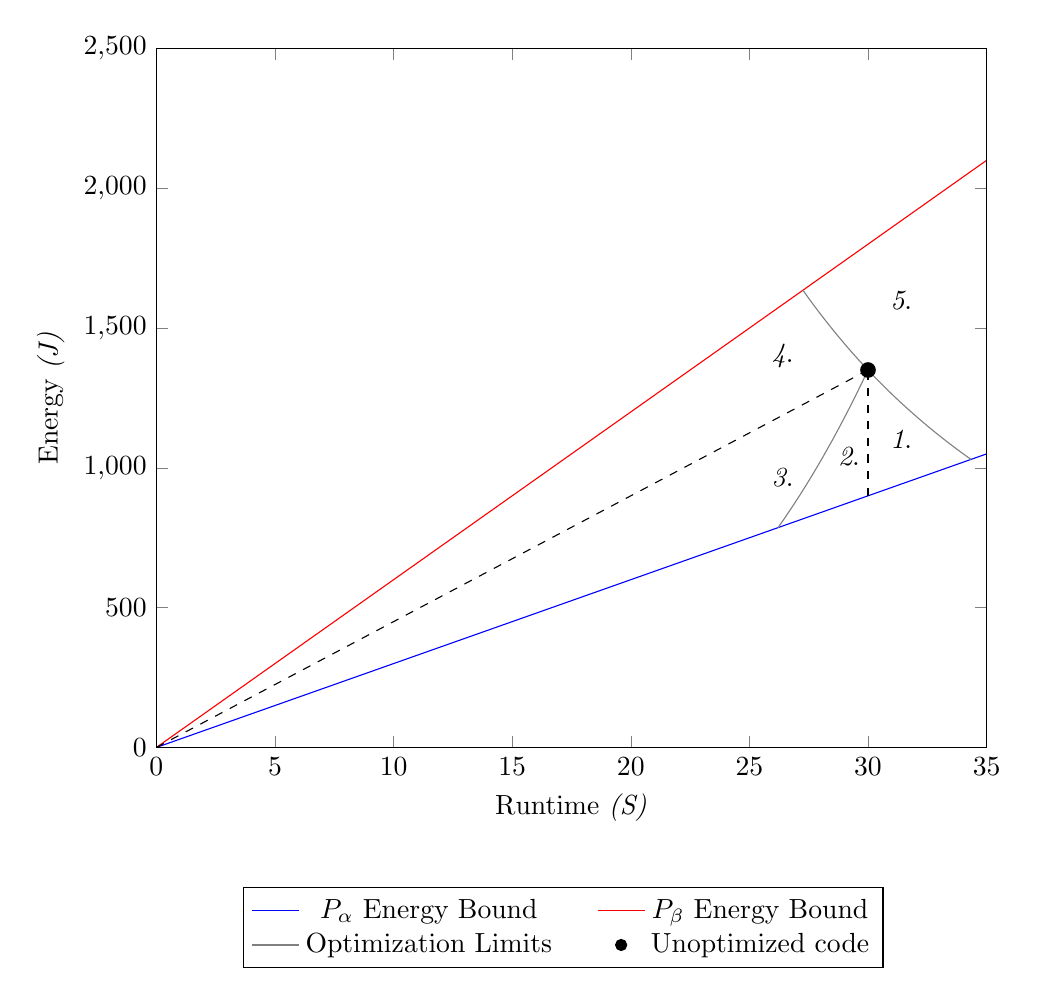
\begin{tikzpicture}
  \begin{axis}[no markers, ylabel={Energy \emph{(J)}}, xlabel={Runtime \emph{(S)}}, axis on top,
    ymin=0, ymax=2500,
    xmin=0, xmax=35,
    width=\linewidth,
    legend style={at={(0.49,-0.2)}, anchor=north,legend columns=2, /tikz/every even column/.append style={column sep=0.5cm}}
    ]

    \pgfmathsetmacro{\baseline}{30}
    \pgfmathsetmacro{\roofline}{60}
    \pgfmathsetmacro{\power}{(\baseline + \roofline) / 2}
    \pgfmathsetmacro{\seconds}{30}
    \pgfmathsetmacro{\energy}{\power * \seconds}
    \pgfmathsetmacro{\baseenergy}{\baseline * \seconds}


    \addplot[domain=\pgfkeysvalueof{/pgfplots/xmin}:\pgfkeysvalueof{/pgfplots/xmax}, blue] {\baseline * x};
    \addlegendentry{$P_{\alpha}$ Energy Bound} 


    \addplot[domain=\pgfkeysvalueof{/pgfplots/xmin}:\pgfkeysvalueof{/pgfplots/xmax}, red] {\roofline * x};
    \addlegendentry{$P_{\beta}$ Energy Bound}

    %ED2P boundaries
    \addlegendentry{Optimization Limits} 

    \addplot[domain=27.25680:34.34143, gray, forget plot] { (\power * \seconds^3) / ((x)^2)};
    \addplot[domain=26.2074:\seconds, gray] { (\power / \seconds^3) * x^4}; % Power time same ratio

    \addlegendimage{only marks, mark=o}
    \addlegendentry{Unoptimized code}


    \addplot[domain=\pgfkeysvalueof{/pgfplots/xmin}:\seconds, dashed] {\power * x};
    \draw[dashed] ({axis cs:\seconds,0}|-{axis cs:0,\baseenergy}) -- ({axis cs:\seconds,0}|-{axis cs:0,\energy});

    \node[circle,fill,inner sep=2pt] at (axis cs:\seconds,\energy) {};
    \node at (axis cs:31.4,1100) {\textit1.};
    \node at (axis cs:29.2,1040) {\textit2.};
    \node at (axis cs:26.4,965) {\textit3.};
    \node at (axis cs:26.4,1400) {\textit4.};
    \node at (axis cs:31.4,1600) {\textit5.};
      
 \end{axis}
\end{tikzpicture}

\caption{Optimization Classifications}\label{fig:pow}
\end{figure}

% All else being equal, energy to solution will reduce if a code can be made to run faster. That said, there is a clear difference between an optimization which specifically targets energy efficiency and this inevitable side-effect of classical optimization.

The definition we have settled on is that the transformation $a \to b$ is a valid power optimization w.r.t a metric $M$ if it is a valid optimization w.r.t. $M$ and the reduction in power draw has a greater impact on improvement in $M$ than any reduction in runtime. Once again, we plot the curve where both two factors have equal effects. All valid power optimizations must lie below this bound.

By plotting the various limits described above we subdivide the performance envelope into three distinct areas corresponding to power optimizations, time optimizations and degraded performance. For the purposes of illustration we add lines of constant time and energy allowing us to subdivide the plot further into the areas labelled:
\begin{enumerate}
\item Power-only optimizations
\item Power-mostly optimizations
\item Time-mostly optimizations
\item Time-only optimizations
\item Code degradation
\end{enumerate}

Between them, areas 1 and 2 represent the section of the performance envelope within which power optimization tools are most capable of identifying potential optimizations. Conventional tools should be used when trying to identify optimizations outside this area. The only parameters required to delineate this space for a given code are values for its runtime and energy costs and knowledge of system baseline power.

Despite its simplicity, this technique offers a surprising wealth of information. Figure \ref{fig:modelpoints} shows the power optimization area we observed when we ran the CFD benchmark of the Rodinia benchmark suite.


\begin{figure}
\label{fig:modelpoints}
 
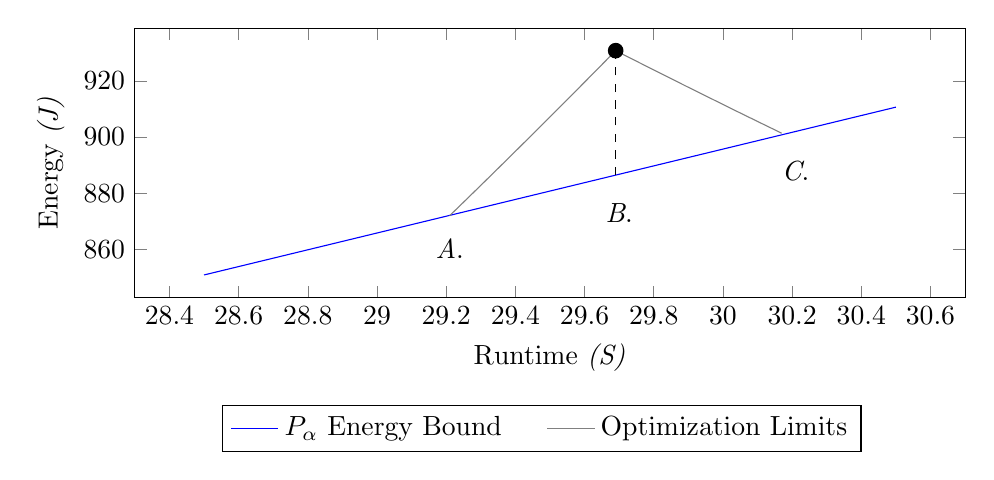
\begin{tikzpicture}
  \begin{axis}[no markers, ylabel={Energy \emph{(J)}}, xlabel={Runtime \emph{(S)}}, axis on top,
    width=\linewidth,
    height=5cm,
    legend style={at={(0.49,-0.4)}, anchor=north,legend columns=2, /tikz/every even column/.append style={column sep=0.5cm}}
    ]

    \pgfmathsetmacro{\baseline}{29.857} % NOP code

    %code, power, time
    %cfd, 31.348872, 29.689872
    %heartwall, 32.072718, 24.456485
    %lavaMD,  32.715703, 65.387028
    %leukocyte, 30.771108, 38.950881
    %streamcluster, 32.192283, 33.801999


     \addplot[domain=28.5:30.5, blue] {\baseline * x};
     \addlegendentry{$P_{\alpha}$ Energy Bound} 

  
     %% CFD %%
     \pgfmathsetmacro{\cfdpower}{31.348872}
     \pgfmathsetmacro{\cfdtime}{29.689872}
     \pgfmathsetmacro{\cfdenergy}{\cfdpower * \cfdtime}
     \pgfmathsetmacro{\baseenergy}{\baseline * \cfdtime}
     \addplot[domain=\cfdtime:30.17, gray, forget plot] { (\cfdpower * \cfdtime^3) / ((x)^2)};
     \addplot[domain=29.21:\cfdtime, gray] { (\cfdpower / \cfdtime^3) * x^4}; % Power time same ratio

     \node[circle,fill,inner sep=2pt] at (axis cs:\cfdtime, \cfdenergy) {};
     \addlegendentry{Optimization Limits} 

    \draw[dashed] ({axis cs:\cfdtime,0}|-{axis cs:0,\baseenergy}) -- ({axis cs:\cfdtime,0}|-{axis cs:0,\cfdenergy});
    
    \node at (axis cs:29.21,860) {\textit A.};                                   
    \node at (axis cs:29.7,873) {\textit B.};                                   
    \node at (axis cs:30.21,888) {\textit C.};                                   



%     %% CFD %%
%     \addplot[domain=39:48, gray] { (\sedtargetenergy * \sedtargetseconds *  \sedtargetseconds) / ((x)^2)};
%     \addplot[domain=33:41, gray] { (\sedtargetpower / \sedtargetseconds^3) * x^4}; % Power time same ratio
%     \addlegendentry{$ED^{2}P$} 
 

    
      
 \end{axis}
\end{tikzpicture}

\caption{Power Heuristic for Rodinia CFD}
\end{figure}

	
	
\todo{Working point}

We first construct a power model in the vein of those proposed in the literature. We then try to link the predictions of our model to the power equations given previously. Essentially we are attempting to test against the null hypothesis - to show how much better or worse our regressed model is better than a naive attempt.


\fragment{this tent shaped region}
\fragment{Despite its simplicity, this simple model provides us with lots of information. \todo{biggest gain to be had by using power vs classical optimization, energy reduction possible through power optimization ignoring any runtime effects, the maximum amount of time we can trade for any gains in energy efficiency, and a convenient way of comparing different codes}}




\fragment{Often power models are assessed by their performance relative to a measured baseline. Although this is important, this figure is somewhat meaningless without context. Our approach is one of quantifying 


\todo{Make this bit less attacky:}
It is also worth noting that this model is effectively useless from a code optimization standpoint as it does not take any software features into account. This property is intentional, as it allows us once again to provide a baseline from which to assess any models. One can only realistically expect to optimize a code to the level at which any changes can be accurately measured. A model which claims to assist in the optimization of codes can only offer optimizations to the extent it shows divergence from this baseline.

}


\fragment{The unknown quantities in our simplified power equations can be empirically measured. \todo{Occam's razor - stronger than regression if not out performed by it}}



\fragment{Accuracy figures without context are notoriously unreliable. To compensate for this we compare the outputs of various models against a baseline we have devised. This baseline consists of what we regard as the simplest non-trivial power model conceivable. This model stands in as a sort of null hypothesis test, our justification being that a complex model only adds value to the extent with which it outperforms this toy model.}

\fragment{Our toy model is not the simplest model possible - It is well established and readily apparent that runtime is the largest contributory factor to power consumption. One could therefore imagine a simple power model}

\fragment{We consider this to be the absolute minimum power consumption possible.}

\fragment{Intentionally simplistic. Our decision to simplify activity factor to active cores is part of this. We assume that instruction pipe-lining does a reasonable job of keeping as much silicon active as possible, and we do not know how much area an individual instruction activates, and a large percentage of power use is from clock circuitry anyway}



\fragment{Two components to our investigation. Firstly, the upper bound imposed by the baseline power consumption. Secondly, as we can only view power figures approximately, the error introduced into these models necessarily limits their usefulness as optimization tools beyond a certain point.}



\begin{table}


\centering
\small
\begin{tabular}{@{}ccccc@{}} \toprule
&\multicolumn{4}{c}{CPU Cores Active} \\ \cmidrule(r){2-5}
Frequency (GHz) & 1 & 2 & 3 & 4 \\ \midrule 
1.60 & 9.180 & 10.970 & 12.832 & 14.555 \\ 
1.70 & 9.449 & 11.446 & 13.295 & 15.112 \\ 
1.80 & 9.592 & 11.654 & 13.617 & 15.682 \\ 
1.90 & 9.816 & 12.009 & 14.168 & 16.291 \\ 
2.10 & 10.272 & 12.709 & 15.161 & 17.605 \\ 
2.20 & 10.559 & 13.161 & 15.705 & 18.333 \\ 
2.30 & 10.812 & 13.551 & 16.419 & 19.070 \\ 
2.40 & 11.303 & 14.290 & 17.012 & 19.946 \\ 
2.50 & 11.680 & 14.784 & 18.000 & 20.837 \\ 
2.60 & 11.819 & 15.144 & 18.616 & 21.879 \\ 
2.70 & 12.205 & 15.830 & 19.379 & 22.940 \\ 
2.90 & 13.095 & 17.196 & 21.155 & 25.344 \\ 
3.00 & 13.547 & 18.160 & 22.210 & 26.759 \\ 
3.10 & 14.048 & 18.870 & 23.639 & 28.284 \\ 
3.20 & 14.504 & 19.726 & 24.940 & 29.857 \\ 
\bottomrule
\end{tabular}
   \vspace{0.5\baselineskip}
\caption{Test Platform Base CPU Power (W)}
\label{tab:baseline}
\end{table} 



\todo{table 2 - benchmark results. Linpack is 35.2428 for 100 seconds}
\todo{Something about how any delta is about how the code uses more logic elements than our NOP lo ops. Our optimization window is therefore within that Delta}

\todo{Be nice, say that this does not invalidate other work, but simply shows that hardware has now reached \reword{convergence} and basically there's little traction left}

Having shown that 

\fragment{This model is not supposed to be rigorous or precise. Rather we present it as the simplest possible non-trivial power model which accounts for the sources of variability in the power equations. In effect our model is functionally equivalent to the power equations
presented previously with appropriate constants substituted \todo{sampled}. We present this model as our null hypothesis - for a model to be useful it must outperform this one. It is necessarily an oversimplification - it ignores clock gating. It should also consistently underestimate the true value, as the benchmark selected intentionally exercises the minimum possible number of logic elements while still performing work.}


\todo{One limitation of this work stems from the nature of RAPL - it is an accumulative measurement of power taking into account all processes. On a loaded system it will measure all tasks }

\begin{figure}
\label{fig:dummy_model}
\includegraphics[width=0.9\linewidth]{./Plots/dummy_model/dummymodel-figure0.pdf}
\caption{Feasible Performance Envelope}
\end{figure}

\todo{Decompose the model - find baseline vs non-baseline components}
\todo{This kind of shows us that the baseline dominates}

\fragment{Limitations to optimizations - the superfluous and the logical equivalences. The first is a no-brainer and boils down to removing unnecessary pre-fetching}

\fragment{Either optimizations which are off the critical path, or else those which are on the critical path }

\fragment{Put another way, any optimization which trades runtime for power has a limited window of}

\todo{equationify fact that energy is power * time, and assume we have power decreases, time static or increases}
\todo{equationify baseline lt optimized lt unoptimized lt roofline} \todo{note - roofline is tdp max}

\todo{Do maths think - by what margin would power have to go down to justify longer runtime? ratio of cost per watt, amortized cost per second}

Nothing discussed so far precludes power optimization in practice.
\todo{imply limits thus far are theoretical}
Even these tight limits may still admit some benefits at extreme scale.
Our final argument however is strictly economic.
\reword{A great deal of attention is paid to the fact that power costs are approaching parity with machine construction costs.} The \choice{implicit, unspoken} \choice{consequence, corollary, implication} being that this has not yet happened. \todo{Ultimate point being here the price difference, machine vs power cost places a further limit on optimization utility. Even if we manage to find a slower, more power efficient method of computing a given result, the cost of energy saved has to be less than the added amortized runtime cost.}


\todo{Legitimate targets for optimization: removing redundant prefetch operations as per phi paper.}
